\chapter{Wall-resolved mesh convergence}
\label{app:zpg:mesh-convergence}

The following wall-normal mesh studies supplement
Section~\ref{sec:evaluation:mesh-families-yplus} for all twelve ZPG cases,
including Huang's three stations. Coefficients are evaluated at each mesh's
\(Re_{\delta2}\)-matched station. Dashed lines show E\c{c}a--Hoekstra
extrapolations from the four finest meshes; shaded bands mark
\(\pm1\%\) of each extrapolated value and do not measure agreement with DNS.

\section{Martin--Duan Parts 2 and 4}

\begin{figure}[!htbp]
    \centering
    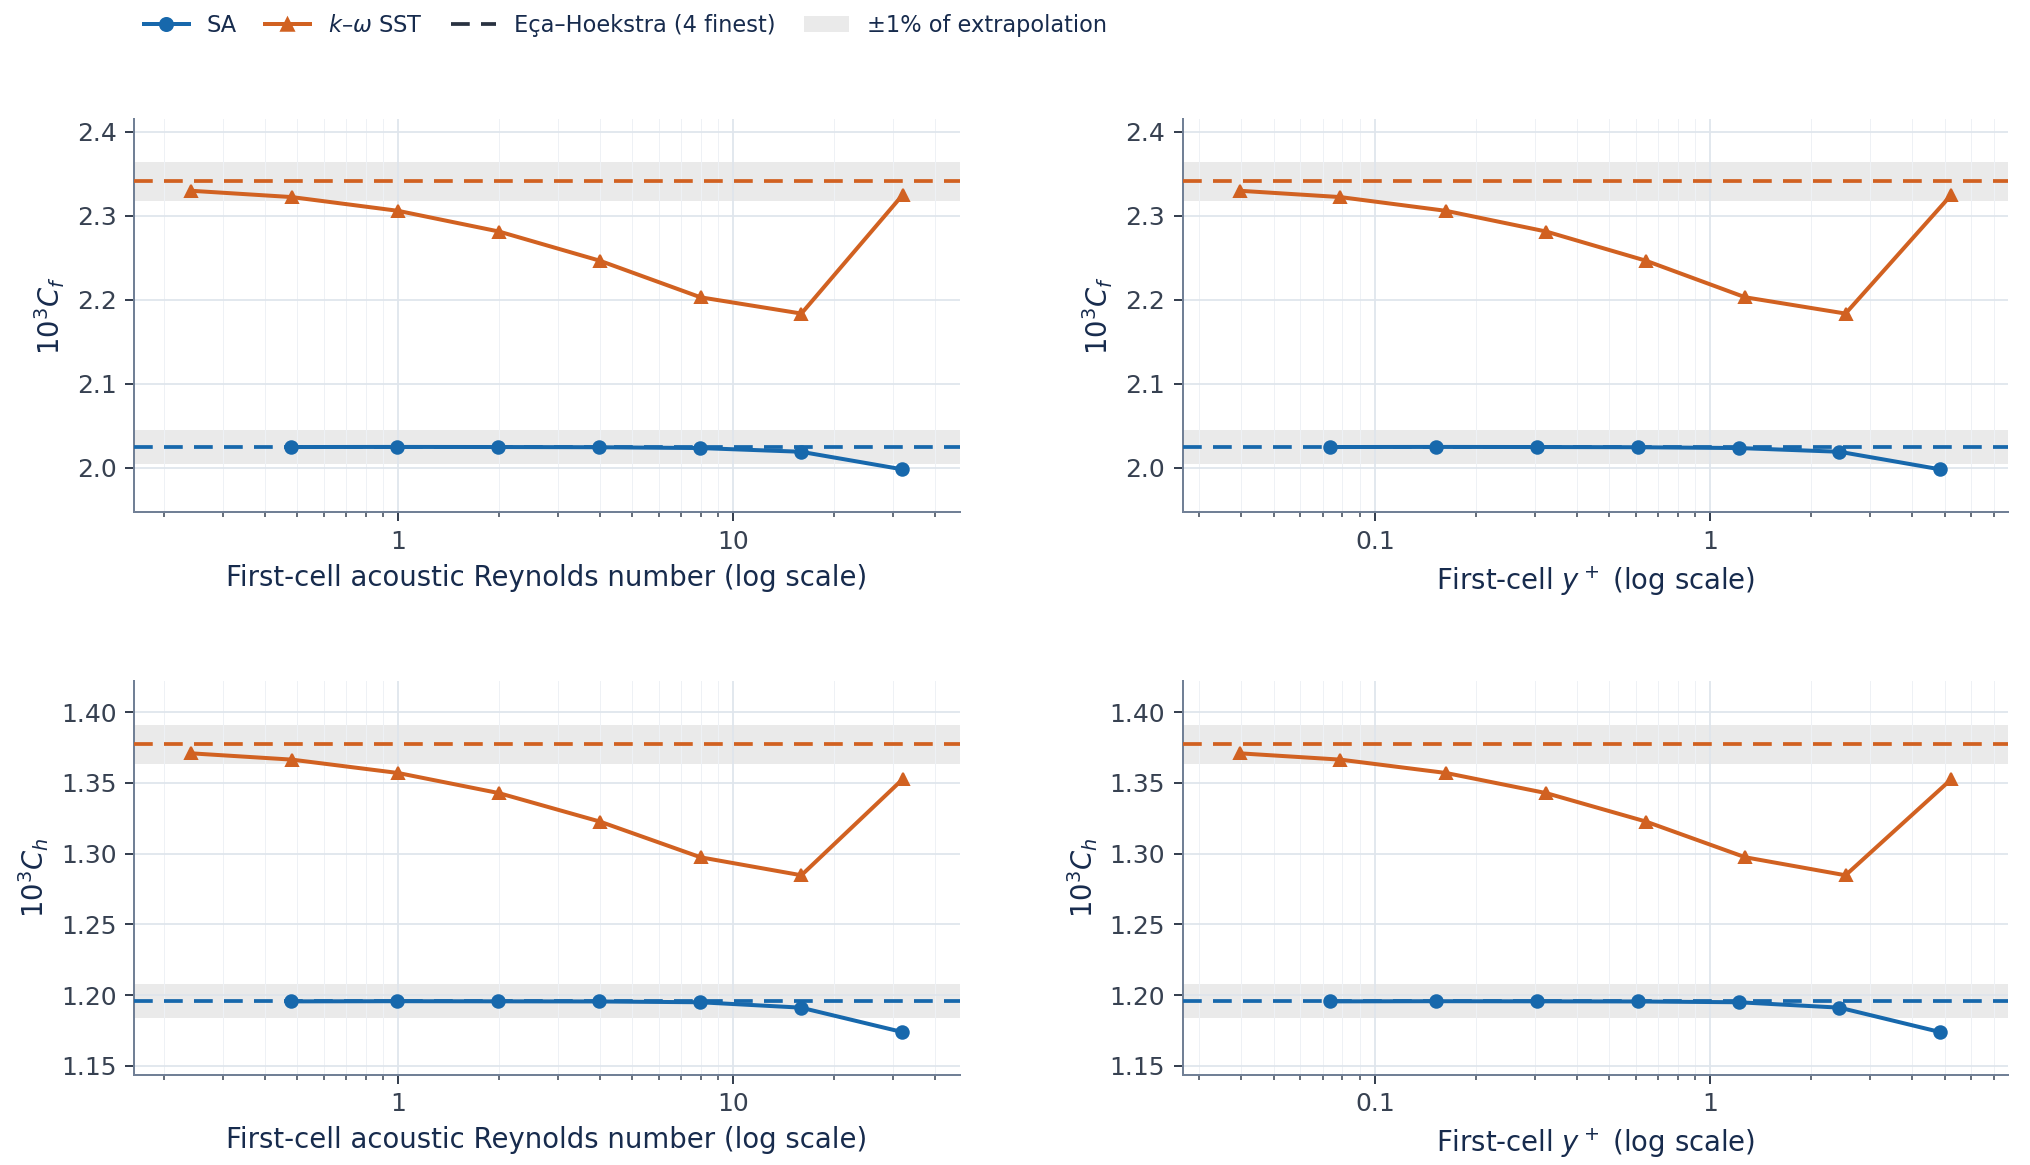
\includegraphics[width=\linewidth]{06_Eval_Methodology/06_Figures/Appendix/Martin_Duan_2_M5T1_Re_delta2.png}
    \caption[Martin--Duan Part~2 M5T1: wall-normal mesh sensitivity]{Wall-normal mesh sensitivity for Martin--Duan Part~2 M5T1, comparing Spalart--Allmaras and \(k\)--\(\omega\) SST. Skin-friction coefficient \(C_f\) (top) and Stanton number \(C_h\) (bottom) versus first-cell acoustic Reynolds number (left) and first-cell \(y^+\) (right) at the matched \(Re_{\delta2}\) = 1538.4 station. Dashed line represents E\c{c}a--Hoekstra extrapolations from the four finest mesh results; shaded bands mark \(\pm1\%\) of each extrapolated value.}
    \label{fig:app:zpg:mesh:M5T1}
\end{figure}

\begin{figure}[!htbp]
    \centering
    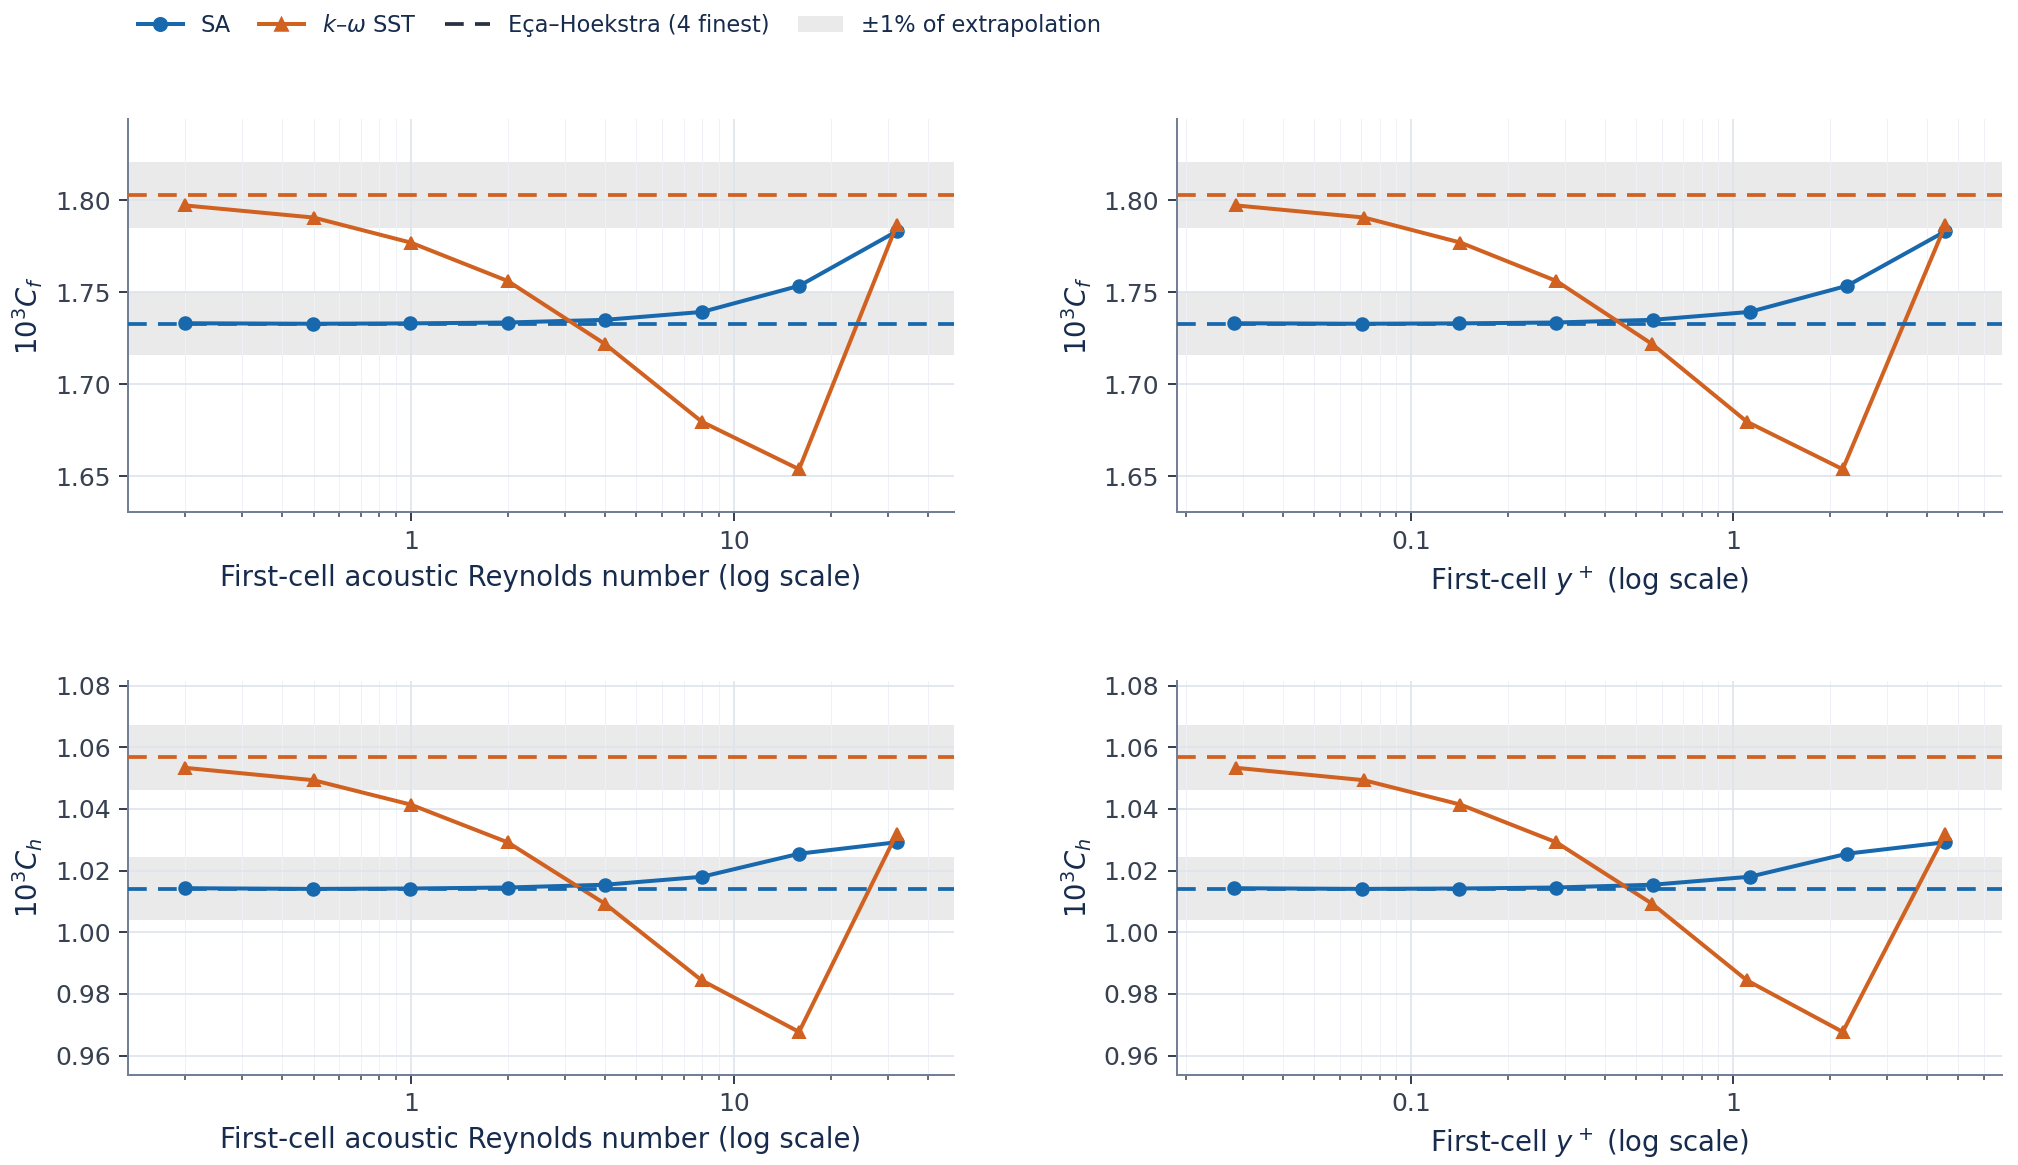
\includegraphics[width=\linewidth]{06_Eval_Methodology/06_Figures/Appendix/Martin_Duan_2_M5T2_Re_delta2.png}
    \caption[Martin--Duan Part~2 M5T2: wall-normal mesh sensitivity]{Wall-normal mesh sensitivity for Martin--Duan Part~2 M5T2, comparing Spalart--Allmaras and \(k\)--\(\omega\) SST. Skin-friction coefficient \(C_f\) (top) and Stanton number \(C_h\) (bottom) versus first-cell acoustic Reynolds number (left) and first-cell \(y^+\) (right) at the matched \(Re_{\delta2}\) = 1521.5 station. Dashed line represents E\c{c}a--Hoekstra extrapolations from the four finest mesh results; shaded bands mark \(\pm1\%\) of each extrapolated value.}
    \label{fig:app:zpg:mesh:M5T2}
\end{figure}

\begin{figure}[!htbp]
    \centering
    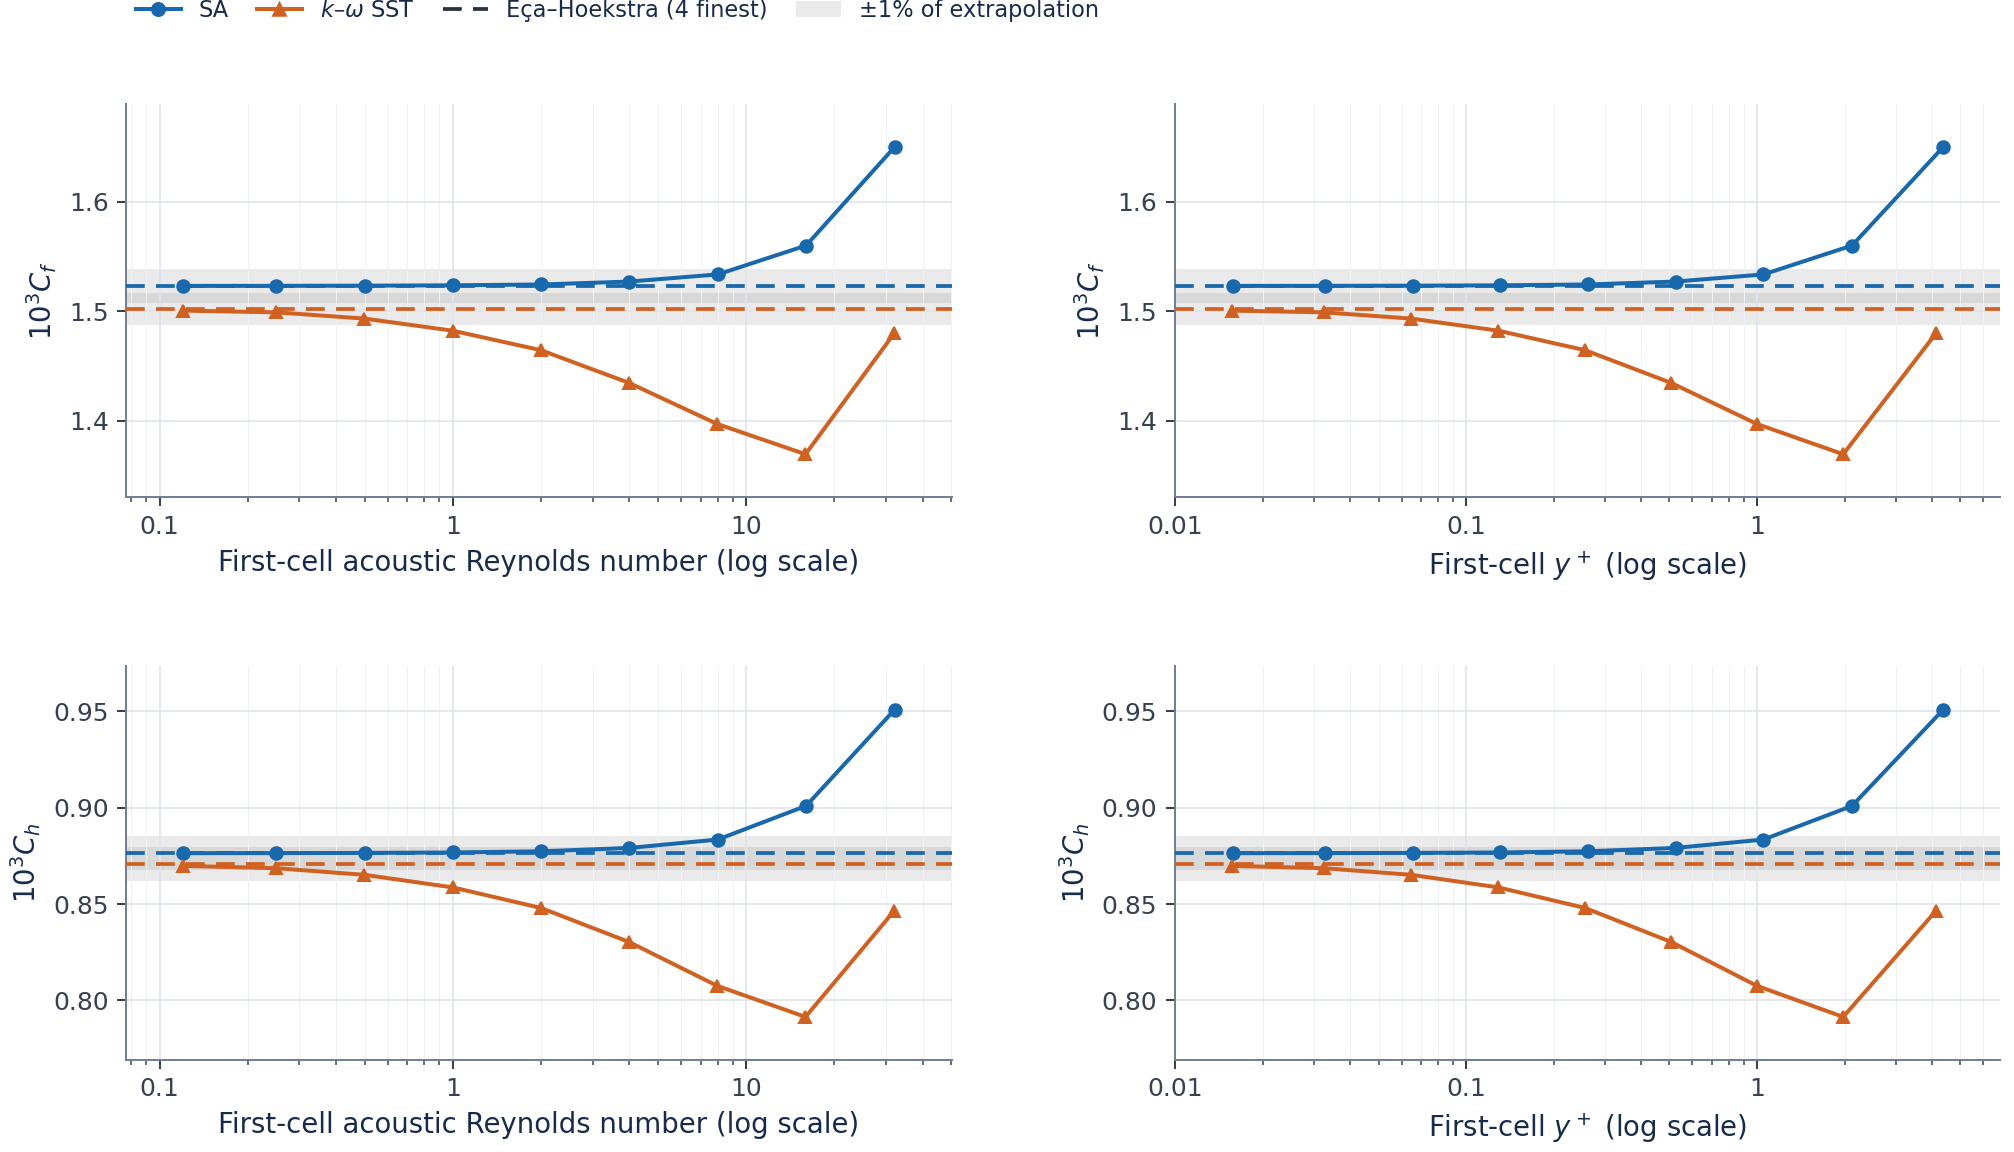
\includegraphics[width=\linewidth]{06_Eval_Methodology/06_Figures/Appendix/Martin_Duan_2_M5T3_Re_delta2.png}
    \caption[Martin--Duan Part~2 M5T3: wall-normal mesh sensitivity]{Wall-normal mesh sensitivity for Martin--Duan Part~2 M5T3, comparing Spalart--Allmaras and \(k\)--\(\omega\) SST. Skin-friction coefficient \(C_f\) (top) and Stanton number \(C_h\) (bottom) versus first-cell acoustic Reynolds number (left) and first-cell \(y^+\) (right) at the matched \(Re_{\delta2}\) = 1524.7 station. Dashed line represents E\c{c}a--Hoekstra extrapolations from the four finest mesh results; shaded bands mark \(\pm1\%\) of each extrapolated value.}
    \label{fig:app:zpg:mesh:M5T3}
\end{figure}

\begin{figure}[!htbp]
    \centering
    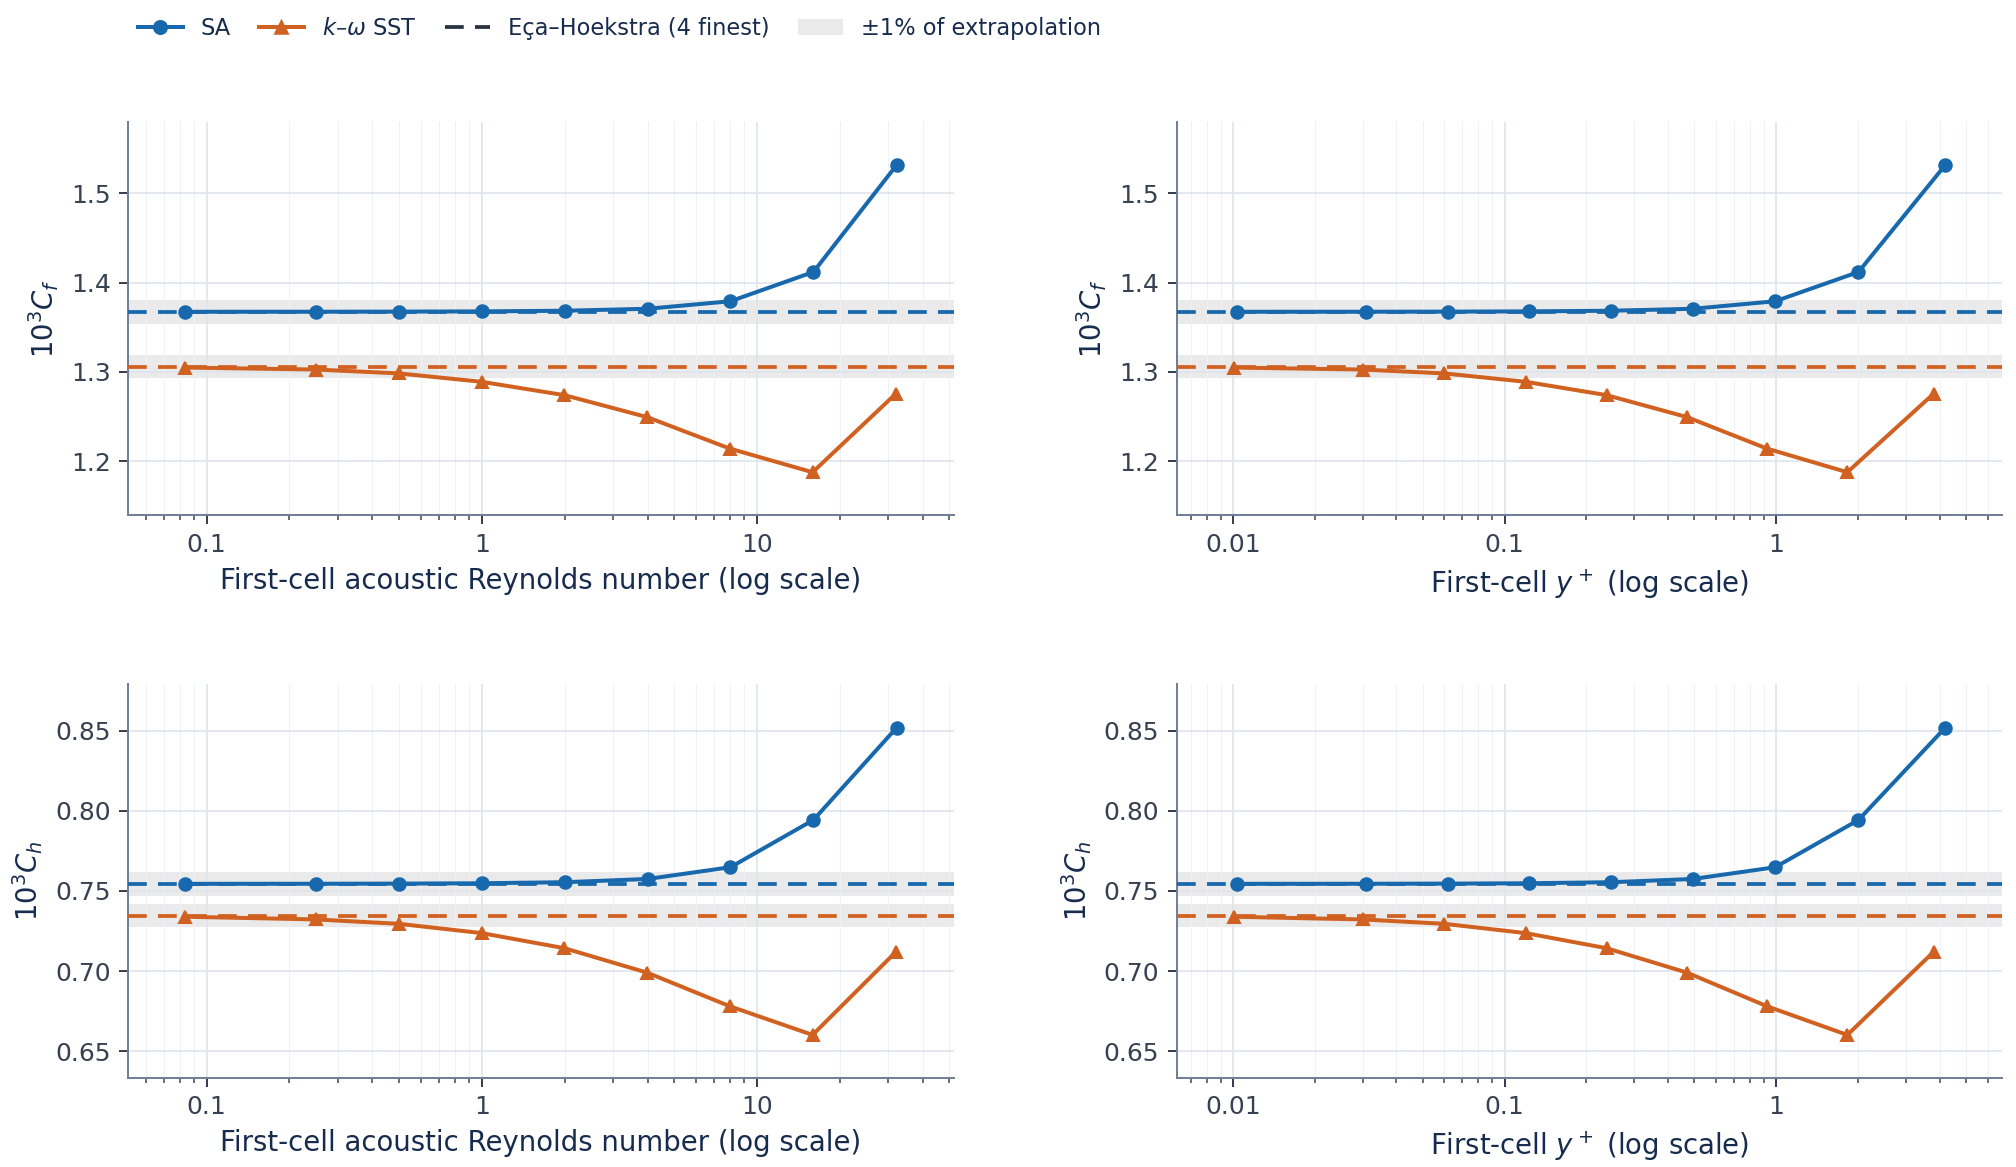
\includegraphics[width=\linewidth]{06_Eval_Methodology/06_Figures/Appendix/Martin_Duan_2_M5T4_Re_delta2.png}
    \caption[Martin--Duan Part~2 M5T4: wall-normal mesh sensitivity]{Wall-normal mesh sensitivity for Martin--Duan Part~2 M5T4, comparing Spalart--Allmaras and \(k\)--\(\omega\) SST. Skin-friction coefficient \(C_f\) (top) and Stanton number \(C_h\) (bottom) versus first-cell acoustic Reynolds number (left) and first-cell \(y^+\) (right) at the matched \(Re_{\delta2}\) = 1526.4 station. Dashed line represents E\c{c}a--Hoekstra extrapolations from the four finest mesh results; shaded bands mark \(\pm1\%\) of each extrapolated value.}
    \label{fig:app:zpg:mesh:M5T4}
\end{figure}

\begin{figure}[!htbp]
    \centering
    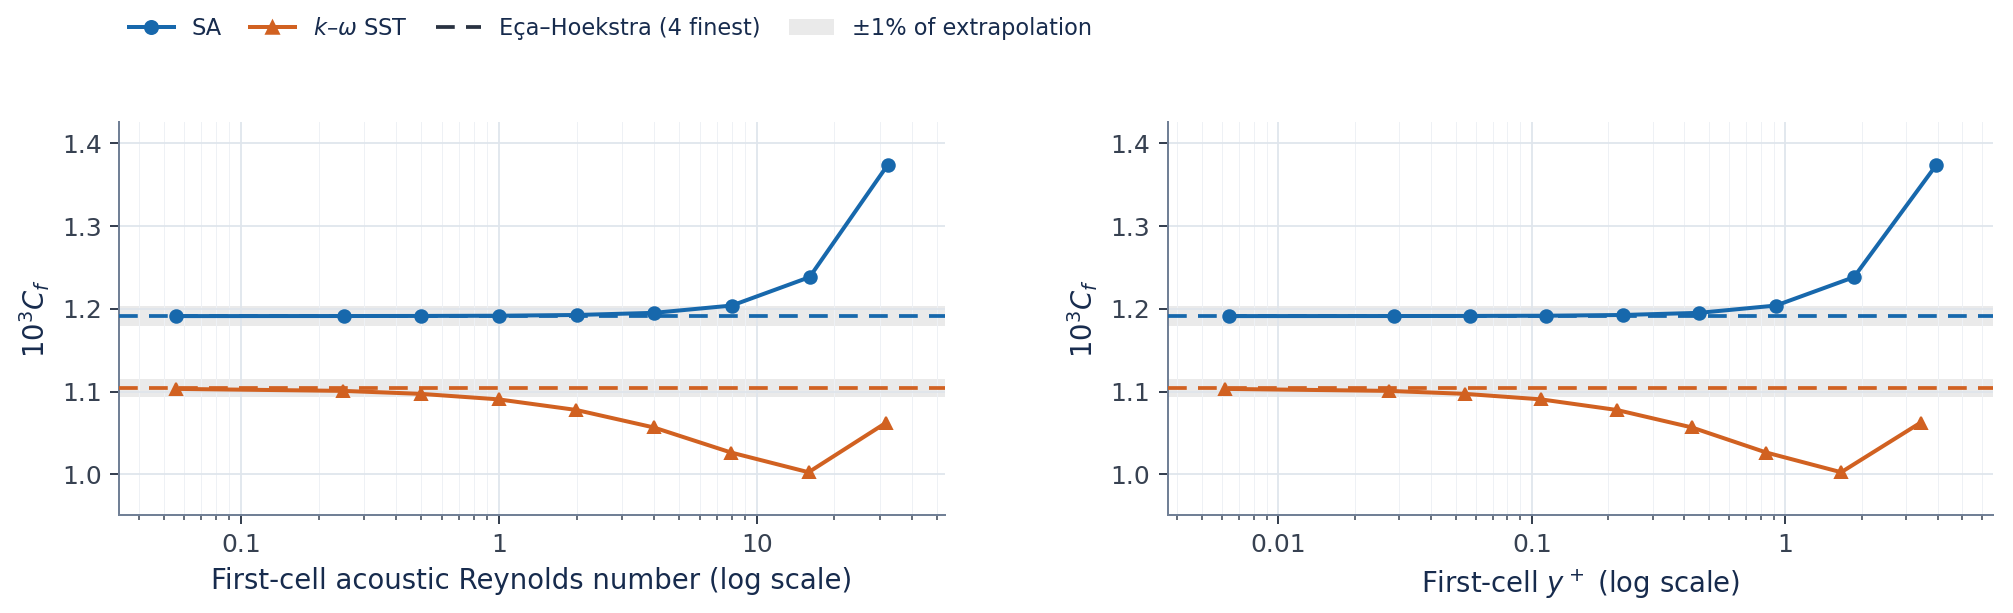
\includegraphics[width=\linewidth]{06_Eval_Methodology/06_Figures/Appendix/Martin_Duan_2_M5T5_Re_delta2.png}
    \caption[Martin--Duan Part~2 M5T5: wall-normal mesh sensitivity]{Wall-normal mesh sensitivity for Martin--Duan Part~2 M5T5, comparing Spalart--Allmaras and \(k\)--\(\omega\) SST. Skin-friction coefficient \(C_f\) versus first-cell acoustic Reynolds number (left) and first-cell \(y^+\) (right) at the matched \(Re_{\delta2}\) = 1536.8 station. Dashed line represents E\c{c}a--Hoekstra extrapolations from the four finest mesh results; shaded bands mark \(\pm1\%\) of each extrapolated value. Heat-transfer is not assessed for this adiabatic case.}
    \label{fig:app:zpg:mesh:M5T5}
\end{figure}

\begin{figure}[!htbp]
    \centering
    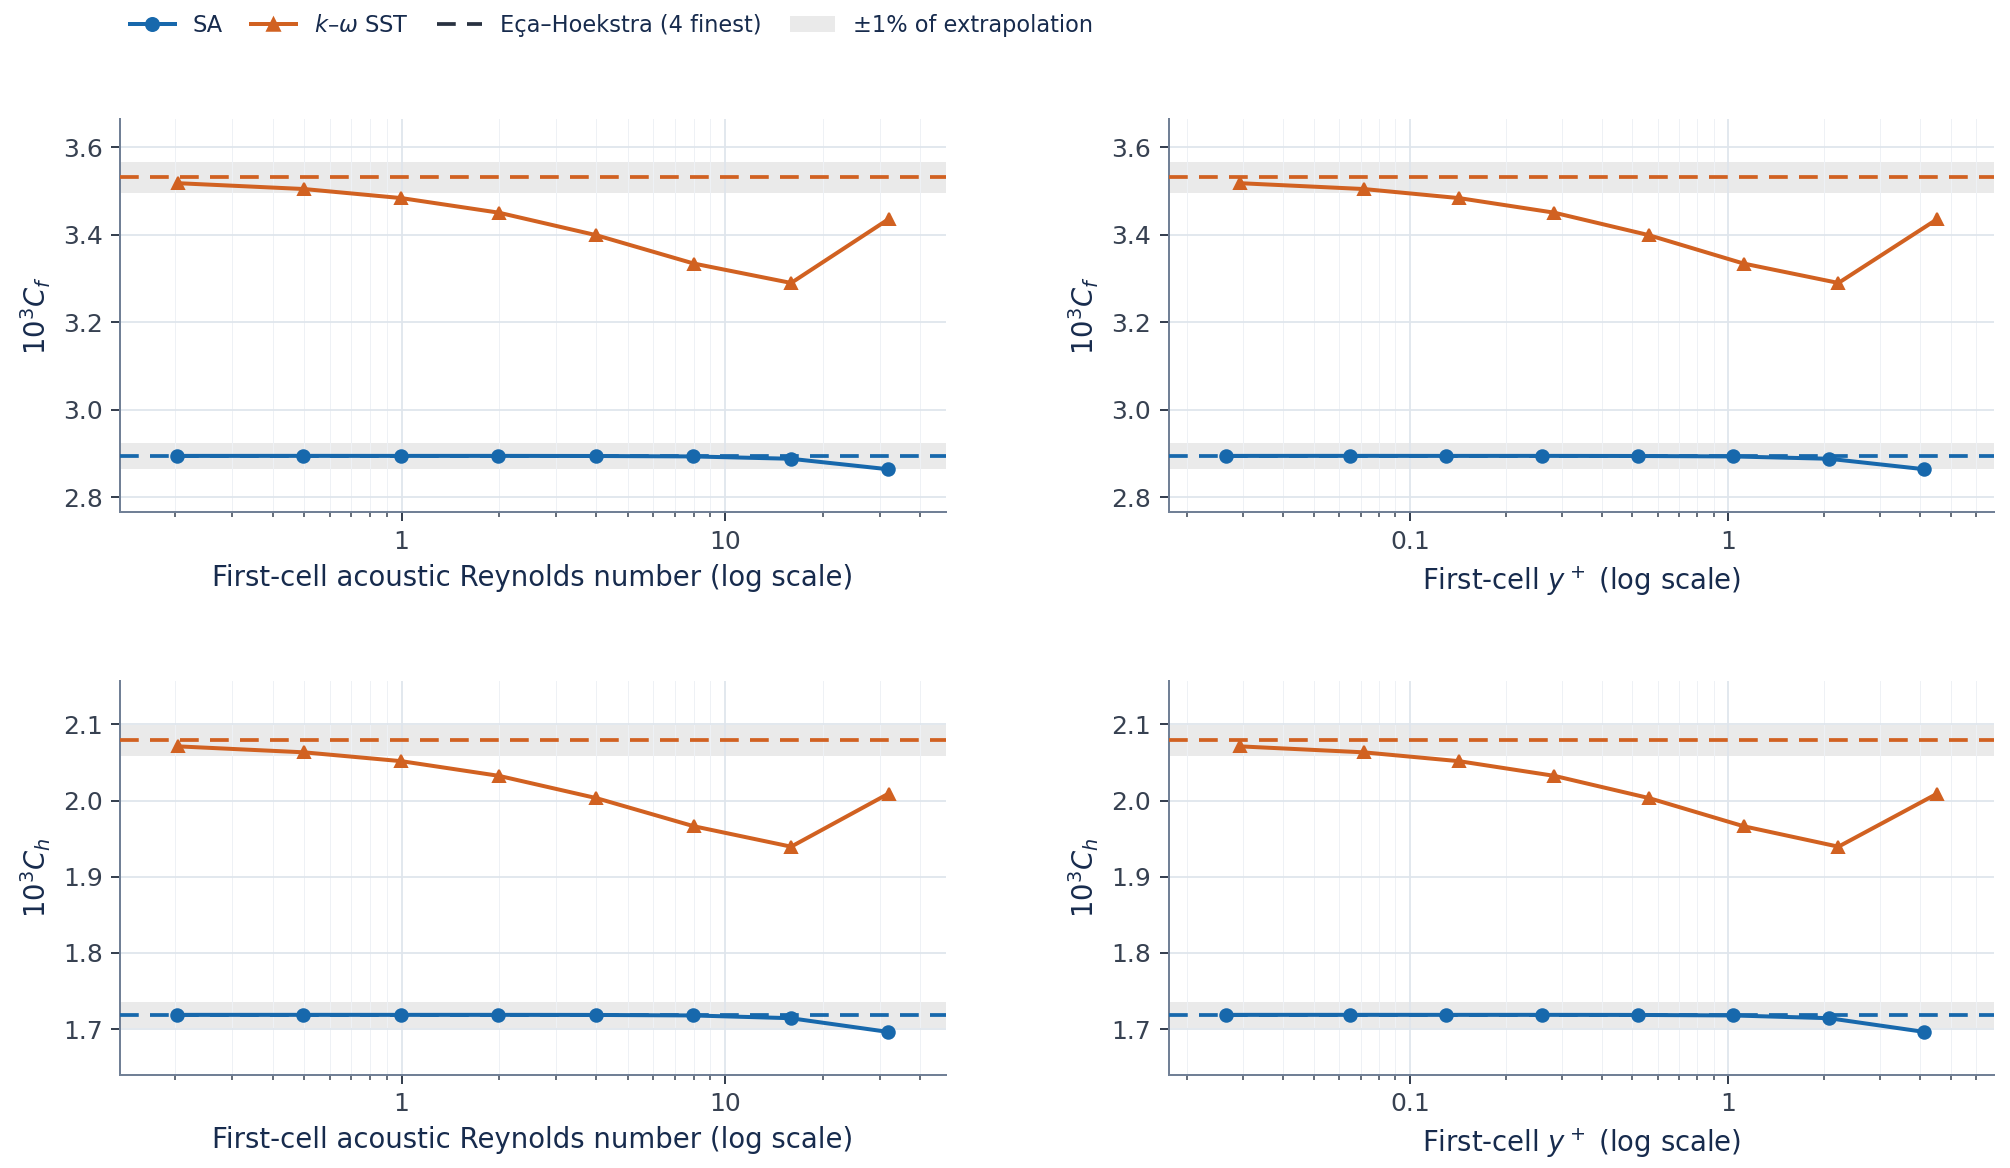
\includegraphics[width=\linewidth]{06_Eval_Methodology/06_Figures/Appendix/Martin_Duan_4_LowH_M3_Re_delta2.png}
    \caption[Martin--Duan Part~4 LowH\_M3: wall-normal mesh sensitivity]{Wall-normal mesh sensitivity for Martin--Duan Part~4 LowH\_M3, comparing Spalart--Allmaras and \(k\)--\(\omega\) SST. Skin-friction coefficient \(C_f\) (top) and Stanton number \(C_h\) (bottom) versus first-cell acoustic Reynolds number (left) and first-cell \(y^+\) (right) at the matched \(Re_{\delta2}\) = 1554.5 station. Dashed line represents E\c{c}a--Hoekstra extrapolations from the four finest mesh results; shaded bands mark \(\pm1\%\) of each extrapolated value.}
    \label{fig:app:zpg:mesh:LowH-M3}
\end{figure}

\clearpage
\section{Zhang cases}

\begin{figure}[!htbp]
    \centering
    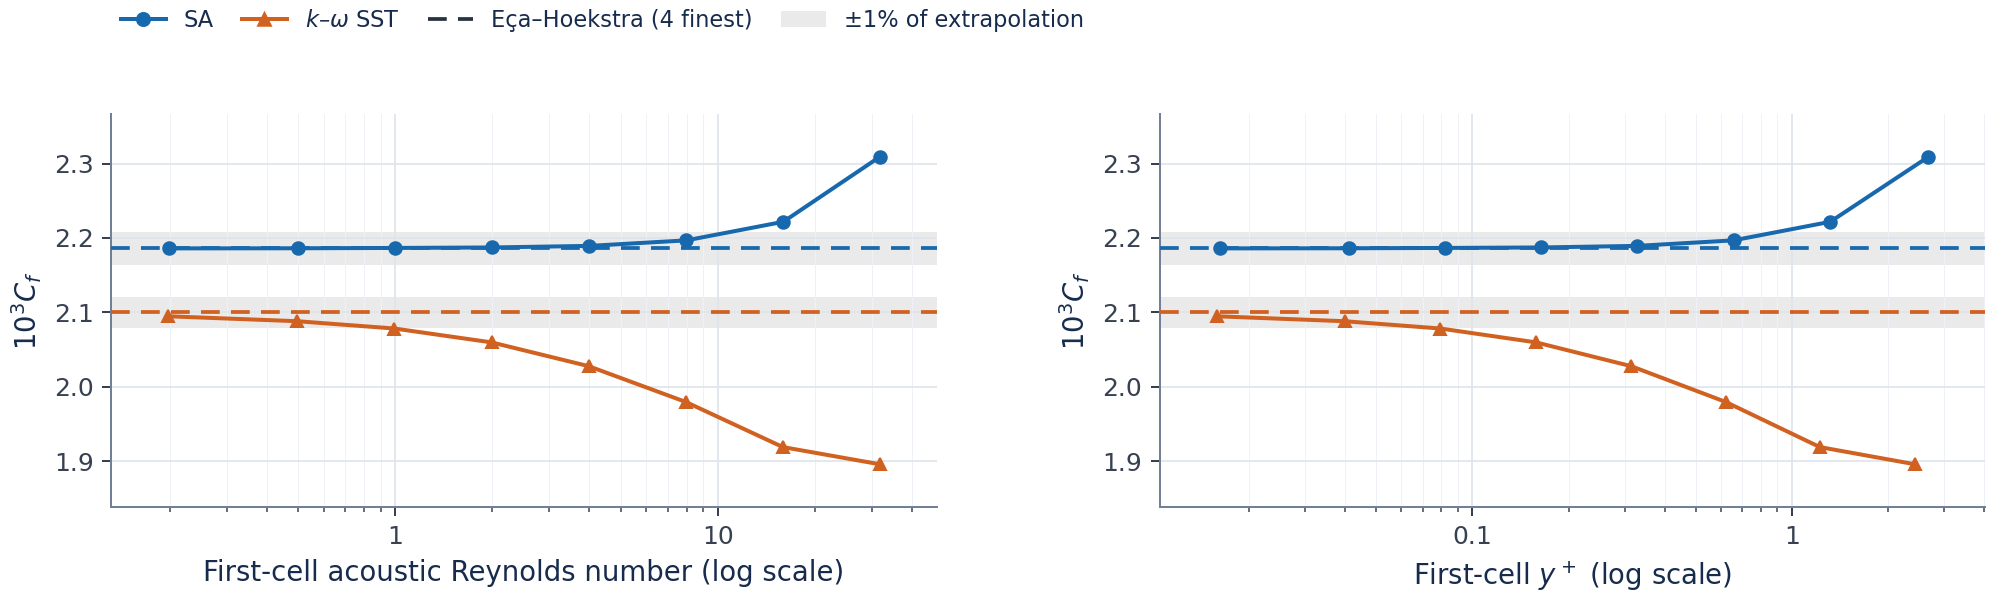
\includegraphics[width=\linewidth]{06_Eval_Methodology/06_Figures/Appendix/Zhang_M2p5_Re_delta2.png}
    \caption[Zhang M2p5: wall-normal mesh sensitivity]{Wall-normal mesh sensitivity for Zhang M2p5, comparing Spalart--Allmaras and \(k\)--\(\omega\) SST. Skin-friction coefficient \(C_f\) versus first-cell acoustic Reynolds number (left) and first-cell \(y^+\) (right) at the matched \(Re_{\delta2}\) = 1657 station. Dashed line represents E\c{c}a--Hoekstra extrapolations from the four finest mesh results; shaded bands mark \(\pm1\%\) of each extrapolated value. Heat-transfer is not assessed for this adiabatic case.}
    \label{fig:app:zpg:mesh:M2p5}
\end{figure}

\begin{figure}[!htbp]
    \centering
    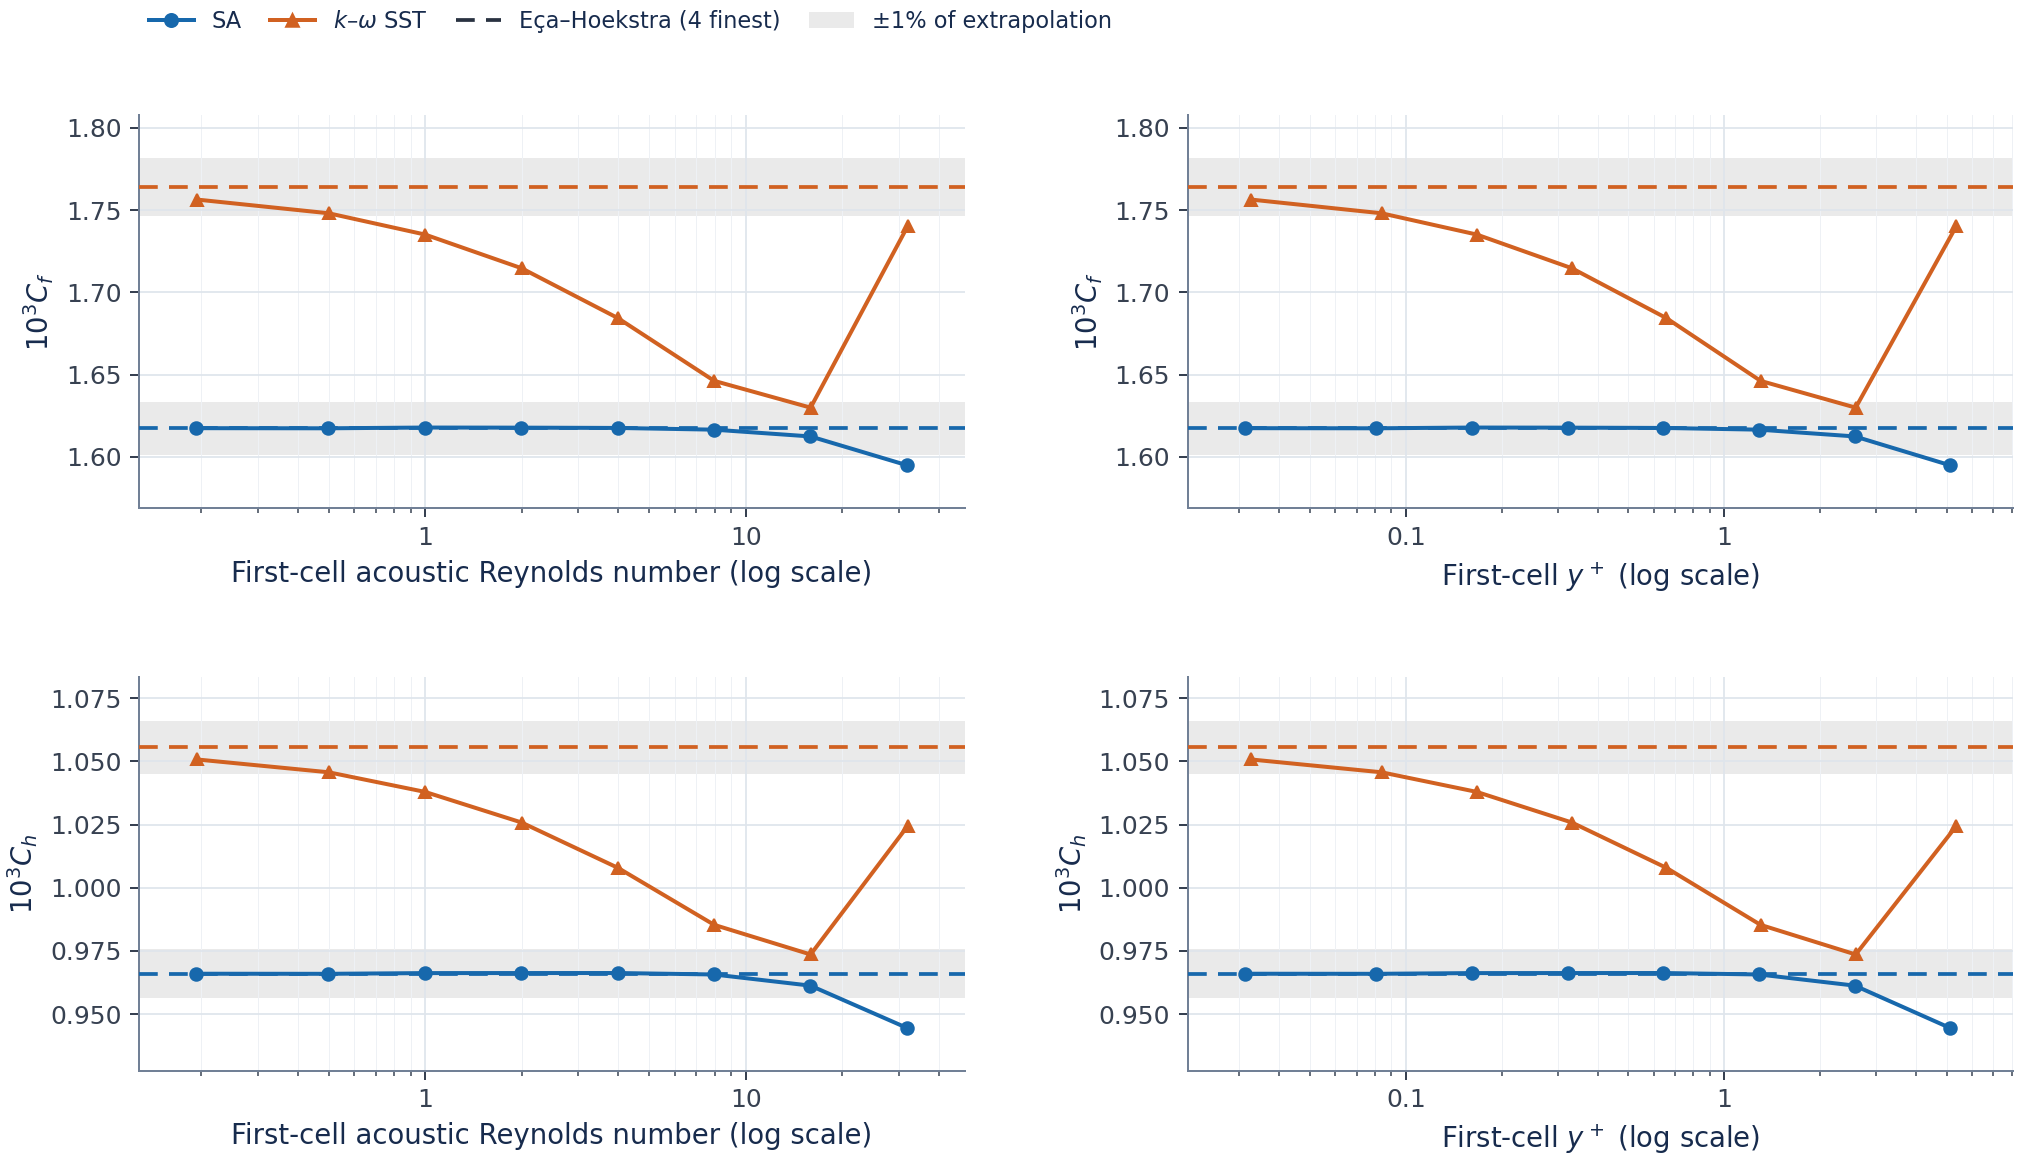
\includegraphics[width=\linewidth]{06_Eval_Methodology/06_Figures/Appendix/Zhang_M6Tw025_Re_delta2.png}
    \caption[Zhang M6Tw025: wall-normal mesh sensitivity]{Wall-normal mesh sensitivity for Zhang M6Tw025, comparing Spalart--Allmaras and \(k\)--\(\omega\) SST. Skin-friction coefficient \(C_f\) (top) and Stanton number \(C_h\) (bottom) versus first-cell acoustic Reynolds number (left) and first-cell \(y^+\) (right) at the matched \(Re_{\delta2}\) = 1135 station. Dashed line represents E\c{c}a--Hoekstra extrapolations from the four finest mesh results; shaded bands mark \(\pm1\%\) of each extrapolated value.}
    \label{fig:app:zpg:mesh:M6Tw025}
\end{figure}

\begin{figure}[!htbp]
    \centering
    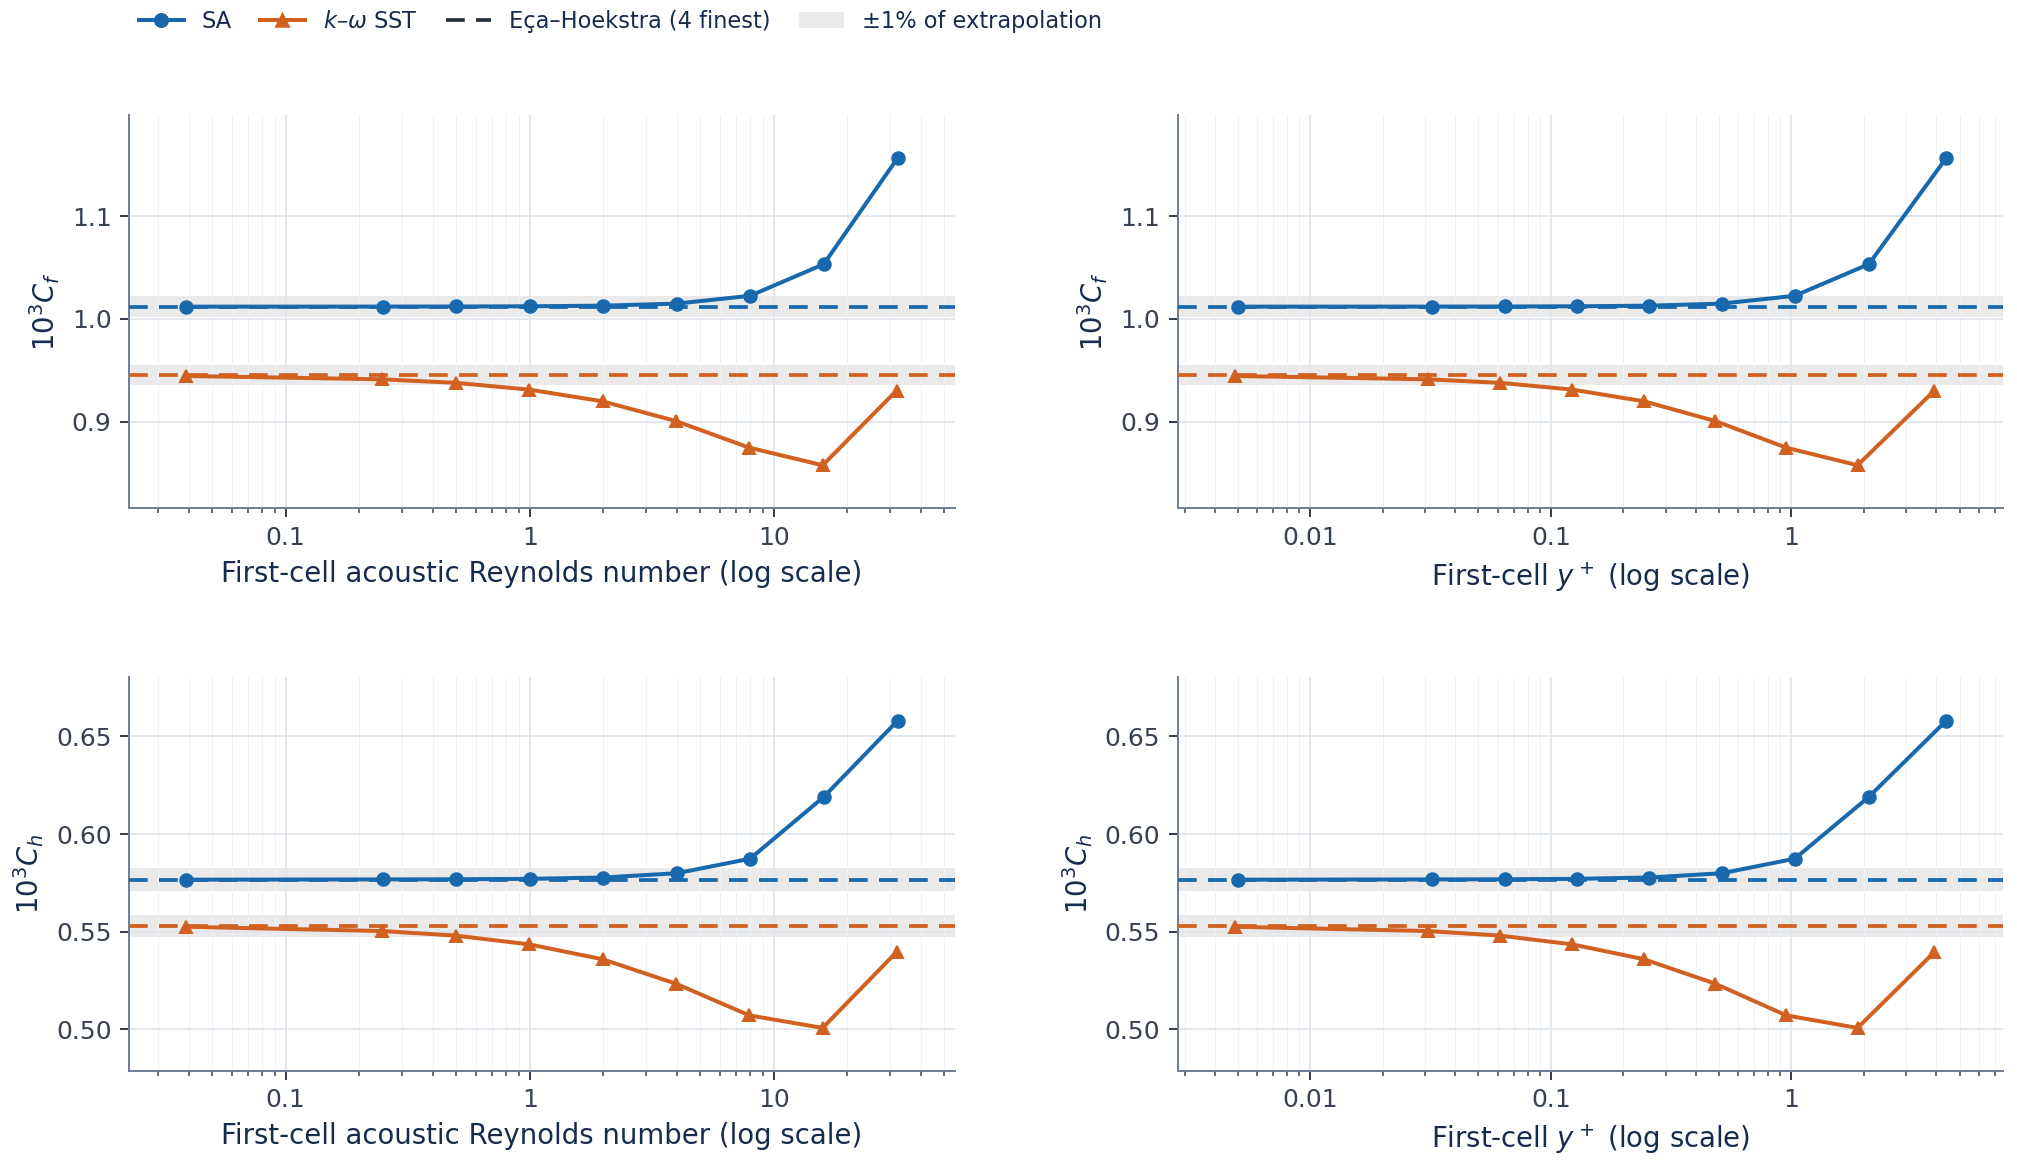
\includegraphics[width=\linewidth]{06_Eval_Methodology/06_Figures/Appendix/Zhang_M6Tw076_Re_delta2.png}
    \caption[Zhang M6Tw076: wall-normal mesh sensitivity]{Wall-normal mesh sensitivity for Zhang M6Tw076, comparing Spalart--Allmaras and \(k\)--\(\omega\) SST. Skin-friction coefficient \(C_f\) (top) and Stanton number \(C_h\) (bottom) versus first-cell acoustic Reynolds number (left) and first-cell \(y^+\) (right) at the matched \(Re_{\delta2}\) = 1746 station. Dashed line represents E\c{c}a--Hoekstra extrapolations from the four finest mesh results; shaded bands mark \(\pm1\%\) of each extrapolated value. The \(C_h\) curves document mesh sensitivity only; the reference-data limitations in Section~\ref{sec:evaluation:benchmark-cases} preclude their use for quantitative heat-flux validation against DNS.}
    \label{fig:app:zpg:mesh:M6Tw076}
\end{figure}

\begin{figure}[!htbp]
    \centering
    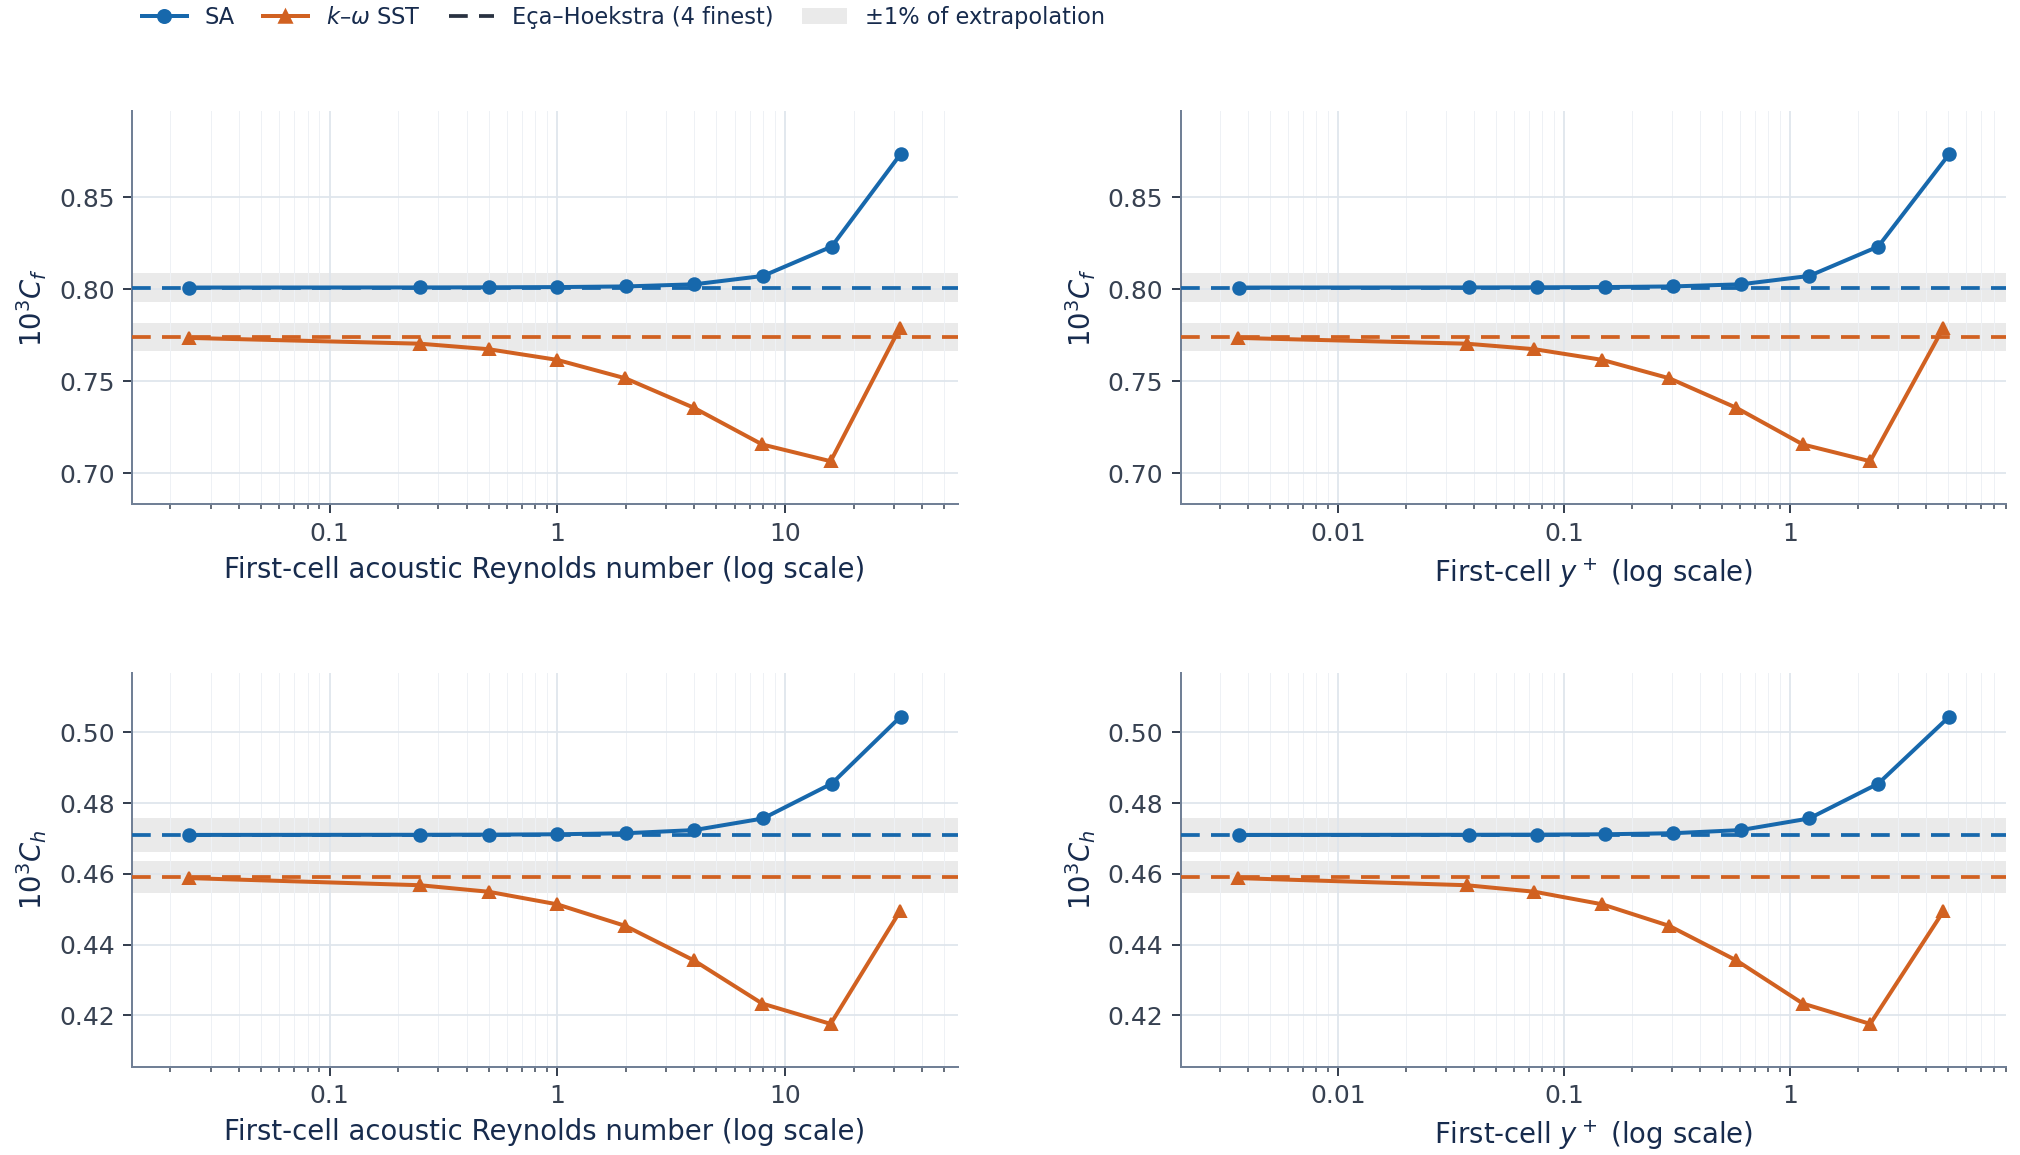
\includegraphics[width=\linewidth]{06_Eval_Methodology/06_Figures/Appendix/Zhang_M8Tw048_Re_delta2.png}
    \caption[Zhang M8Tw048: wall-normal mesh sensitivity]{Wall-normal mesh sensitivity for Zhang M8Tw048, comparing Spalart--Allmaras and \(k\)--\(\omega\) SST. Skin-friction coefficient \(C_f\) (top) and Stanton number \(C_h\) (bottom) versus first-cell acoustic Reynolds number (left) and first-cell \(y^+\) (right) at the matched \(Re_{\delta2}\) = 1990 station. Dashed line represents E\c{c}a--Hoekstra extrapolations from the four finest mesh results; shaded bands mark \(\pm1\%\) of each extrapolated value.}
    \label{fig:app:zpg:mesh:M8Tw048}
\end{figure}

\begin{figure}[!htbp]
    \centering
    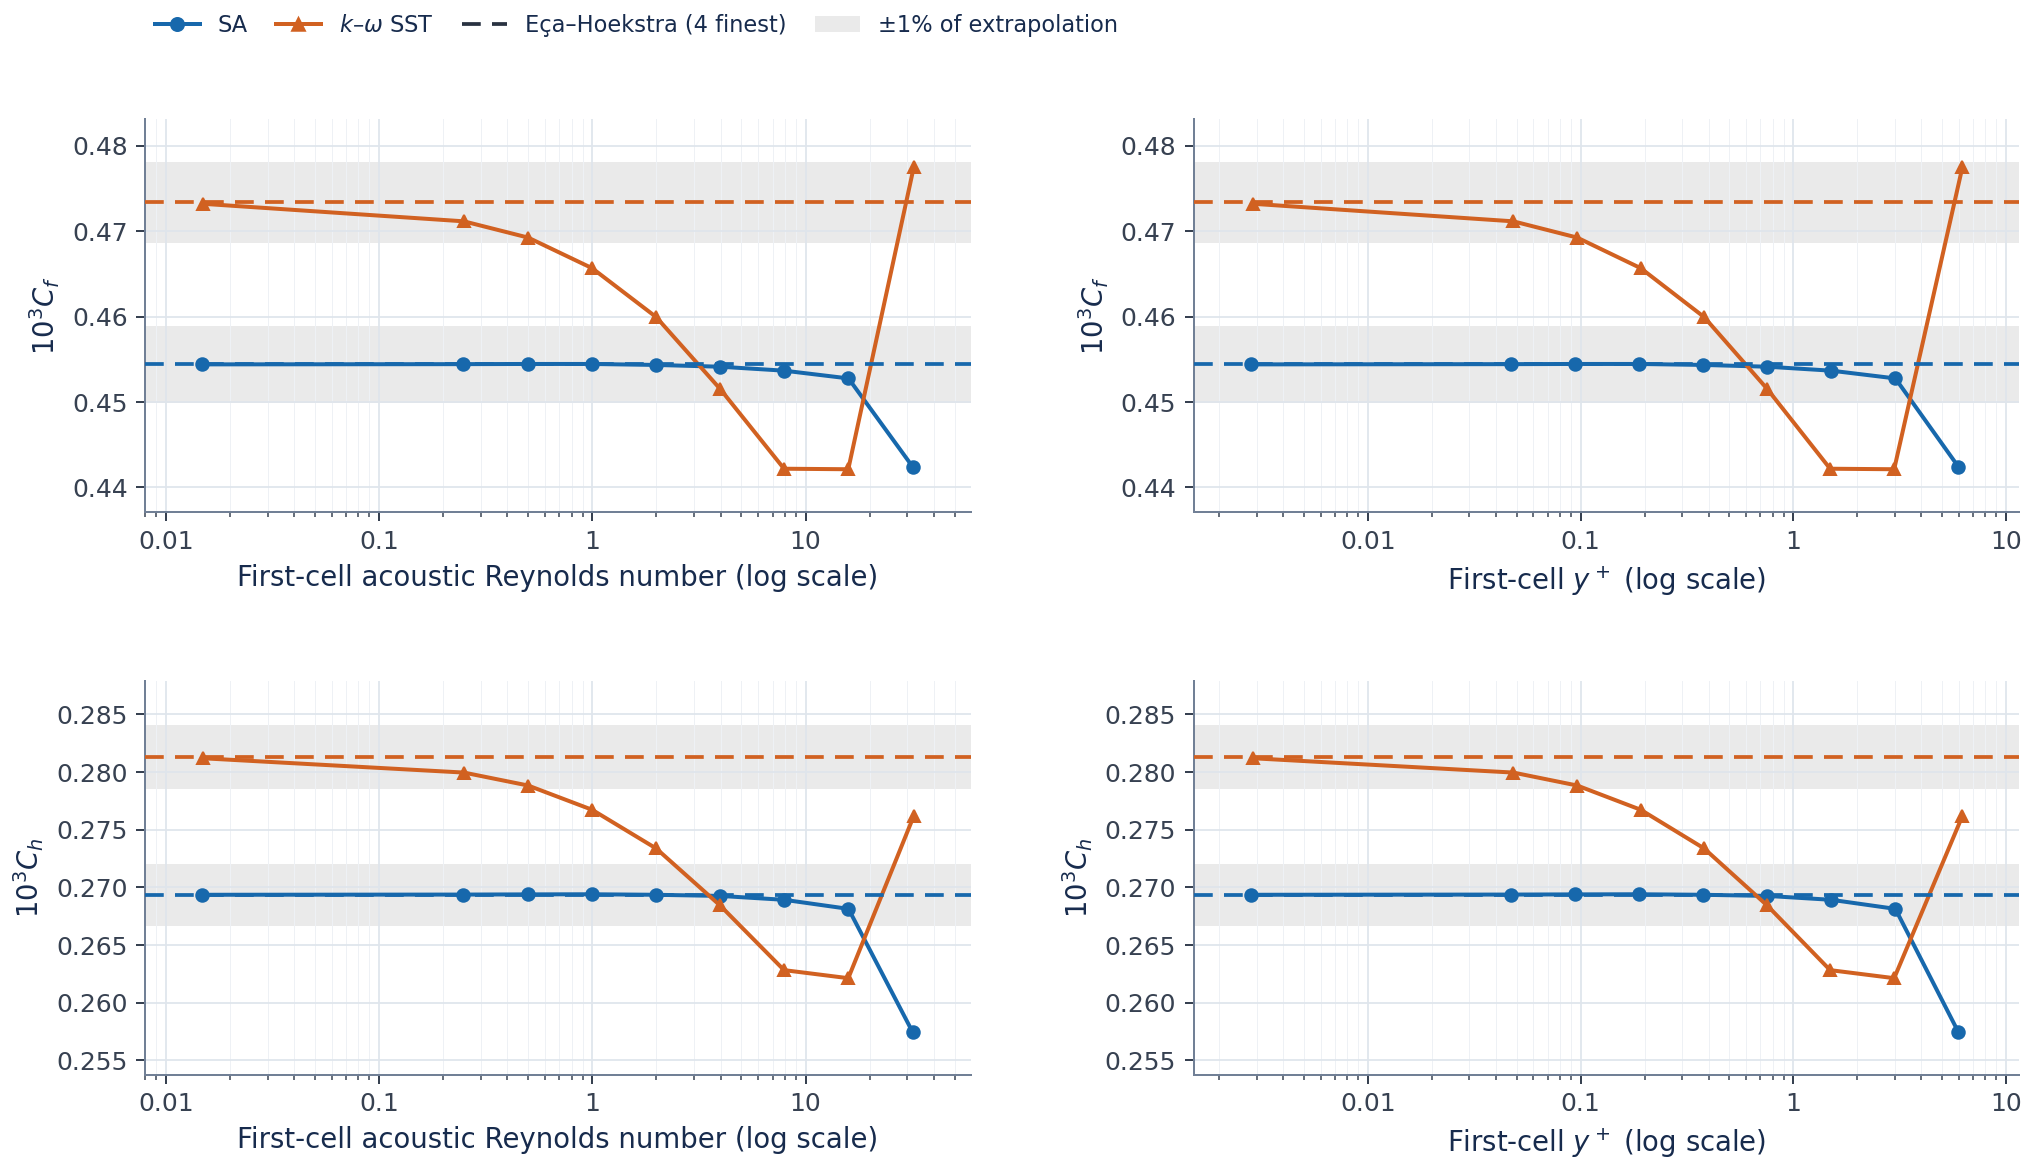
\includegraphics[width=\linewidth]{06_Eval_Methodology/06_Figures/Appendix/Zhang_M14Tw018_Re_delta2.png}
    \caption[Zhang M14Tw018: wall-normal mesh sensitivity]{Wall-normal mesh sensitivity for Zhang M14Tw018, comparing Spalart--Allmaras and \(k\)--\(\omega\) SST. Skin-friction coefficient \(C_f\) (top) and Stanton number \(C_h\) (bottom) versus first-cell acoustic Reynolds number (left) and first-cell \(y^+\) (right) at the matched \(Re_{\delta2}\) = 2354 station. Dashed line represents E\c{c}a--Hoekstra extrapolations from the four finest mesh results; shaded bands mark \(\pm1\%\) of each extrapolated value.}
    \label{fig:app:zpg:mesh:M14Tw018}
\end{figure}

\clearpage
\section{Huang case at stations BL1--BL3}

\begin{figure}[!htbp]
    \centering
    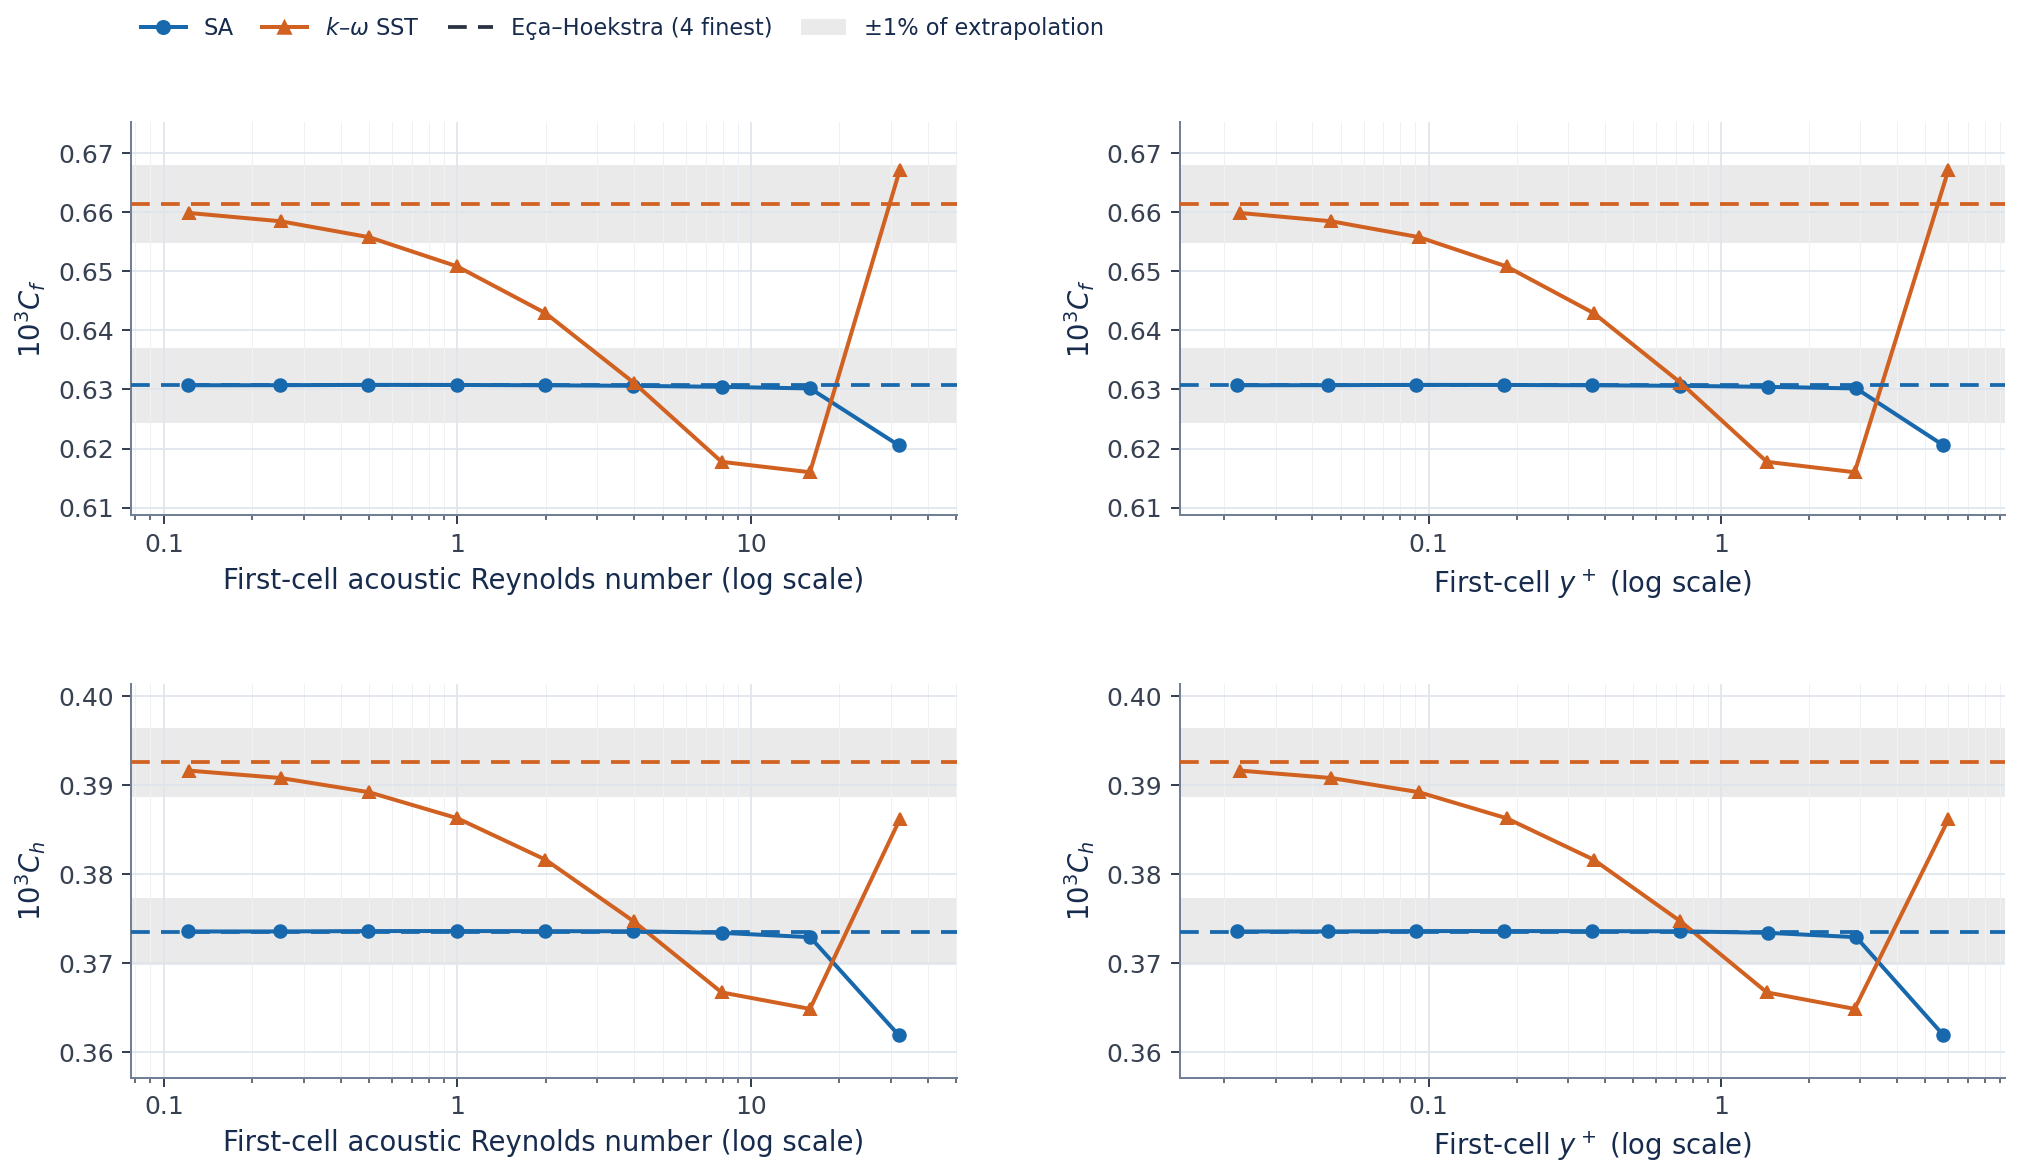
\includegraphics[width=\linewidth]{06_Eval_Methodology/06_Figures/Appendix/Huang_M11Tw20_BL1.png}
    \caption[Huang M11Tw020 at station BL1: wall-normal mesh sensitivity]{Wall-normal mesh sensitivity for Huang M11Tw020 at station BL1, comparing Spalart--Allmaras and \(k\)--\(\omega\) SST. Skin-friction coefficient \(C_f\) (top) and Stanton number \(C_h\) (bottom) versus first-cell acoustic Reynolds number (left) and first-cell \(y^+\) (right) at the matched \(Re_{\delta2}\) = 2204 station. Dashed line represents E\c{c}a--Hoekstra extrapolations from the four finest mesh results; shaded bands mark \(\pm1\%\) of each extrapolated value.}
    \label{fig:app:zpg:mesh:Huang-BL1}
\end{figure}

\begin{figure}[!htbp]
    \centering
    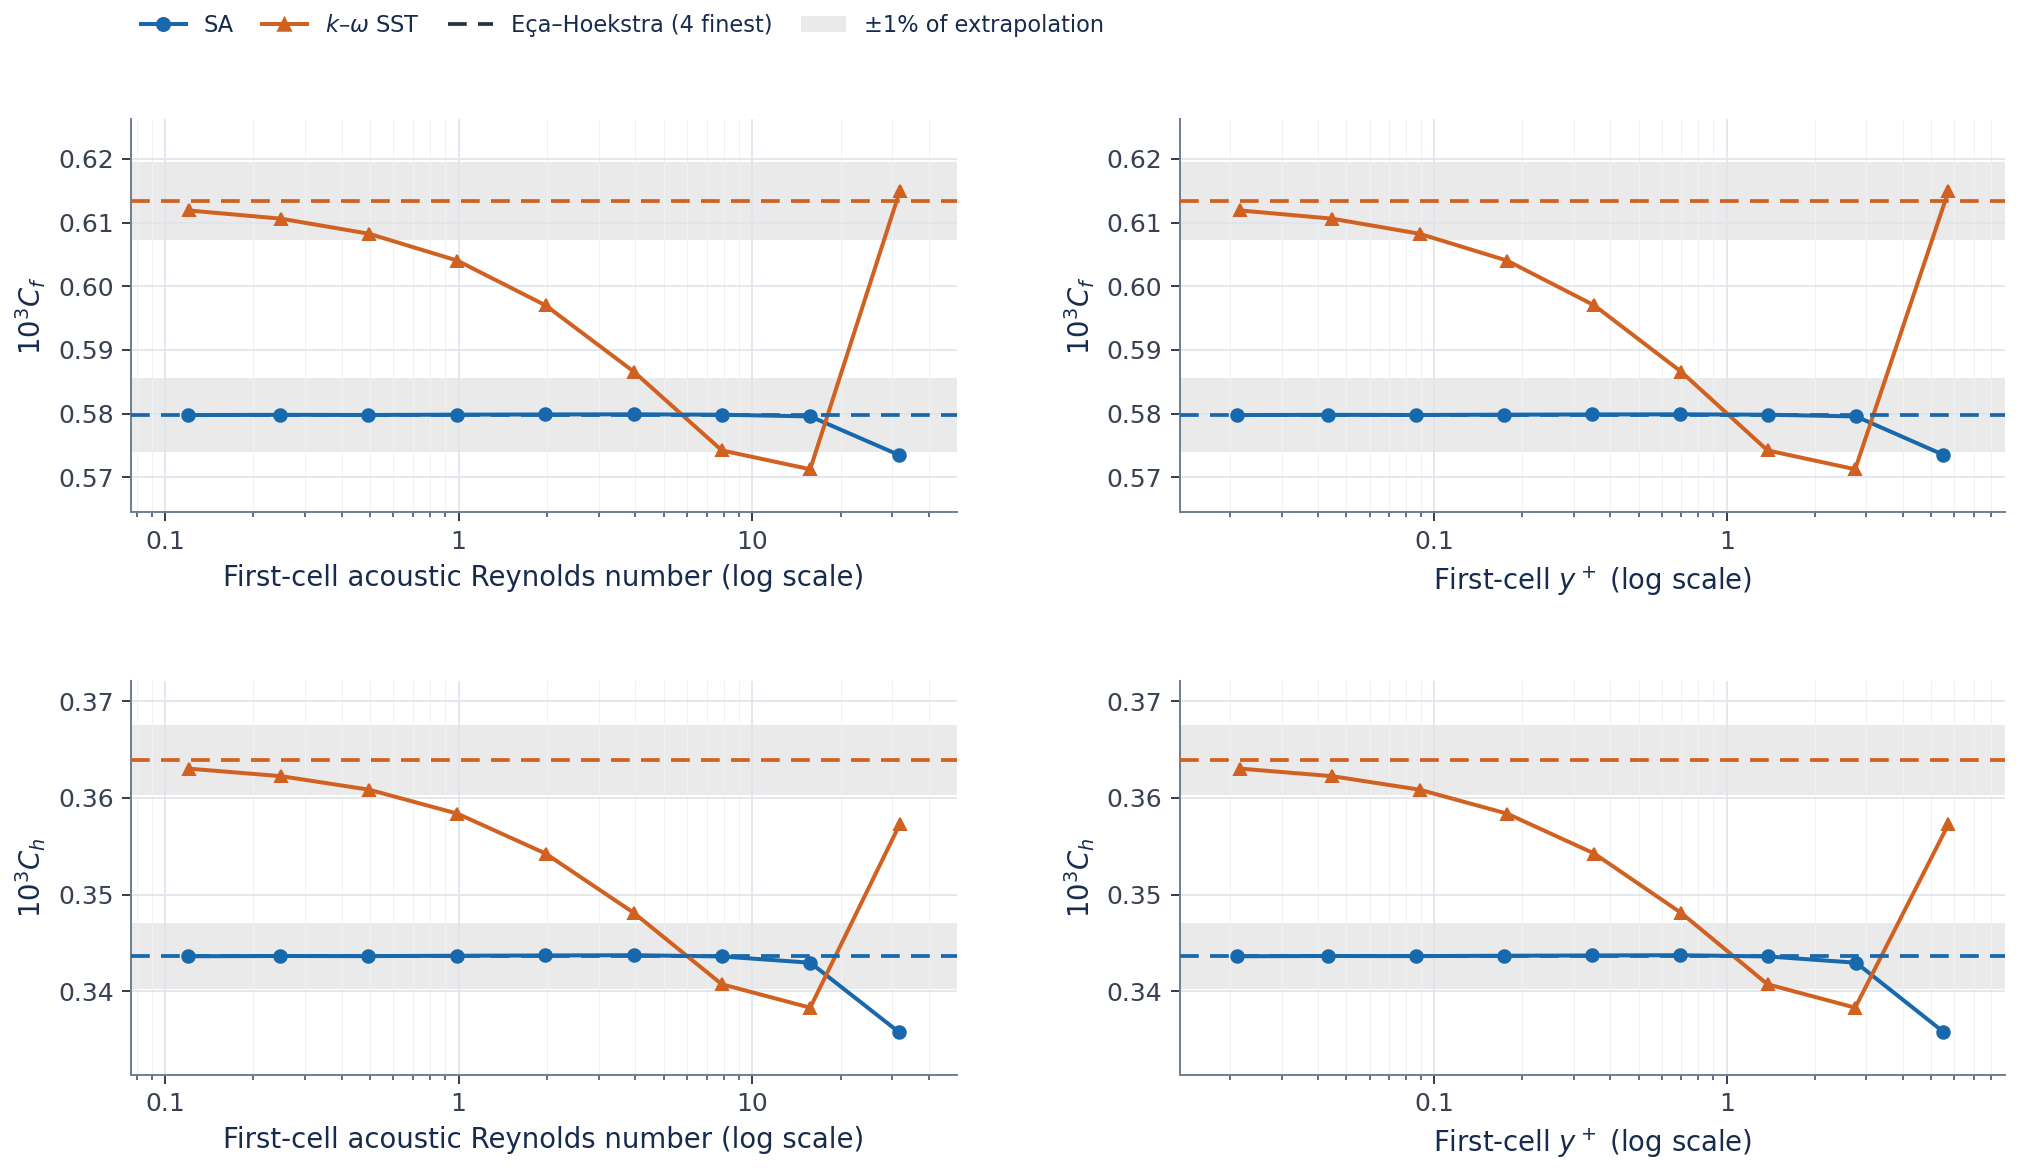
\includegraphics[width=\linewidth]{06_Eval_Methodology/06_Figures/Appendix/Huang_M11Tw20_BL2.png}
    \caption[Huang M11Tw020 at station BL2: wall-normal mesh sensitivity]{Wall-normal mesh sensitivity for Huang M11Tw020 at station BL2, comparing Spalart--Allmaras and \(k\)--\(\omega\) SST. Skin-friction coefficient \(C_f\) (top) and Stanton number \(C_h\) (bottom) versus first-cell acoustic Reynolds number (left) and first-cell \(y^+\) (right) at the matched \(Re_{\delta2}\) = 3419 station. Dashed line represents E\c{c}a--Hoekstra extrapolations from the four finest mesh results; shaded bands mark \(\pm1\%\) of each extrapolated value.}
    \label{fig:app:zpg:mesh:Huang-BL2}
\end{figure}

\begin{figure}[!htbp]
    \centering
    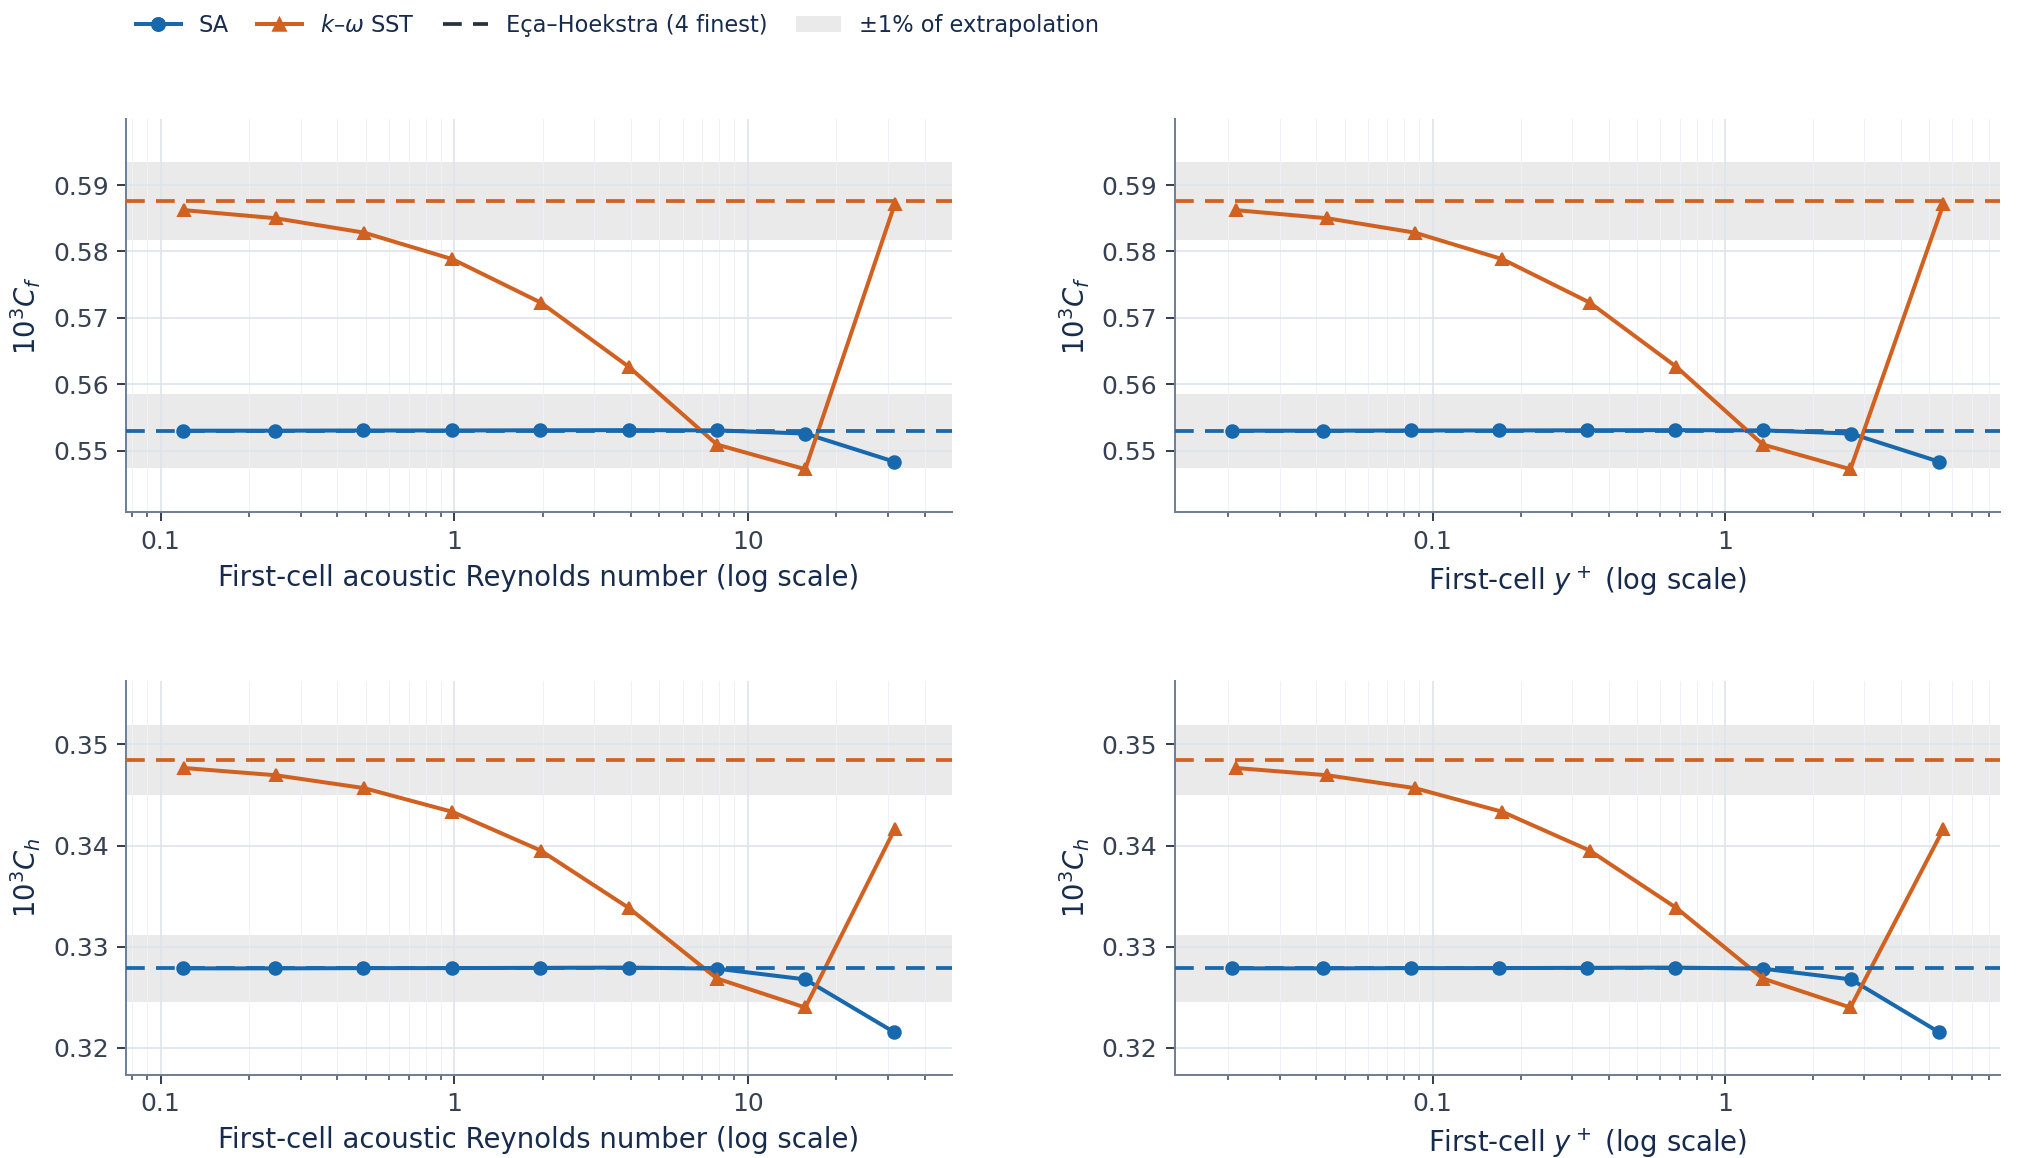
\includegraphics[width=\linewidth]{06_Eval_Methodology/06_Figures/Appendix/Huang_M11Tw20_BL3.png}
    \caption[Huang M11Tw020 at station BL3: wall-normal mesh sensitivity]{Wall-normal mesh sensitivity for Huang M11Tw020 at station BL3, comparing Spalart--Allmaras and \(k\)--\(\omega\) SST. Skin-friction coefficient \(C_f\) (top) and Stanton number \(C_h\) (bottom) versus first-cell acoustic Reynolds number (left) and first-cell \(y^+\) (right) at the matched \(Re_{\delta2}\) = 4390 station. Dashed line represents E\c{c}a--Hoekstra extrapolations from the four finest mesh results; shaded bands mark \(\pm1\%\) of each extrapolated value.}
    \label{fig:app:zpg:mesh:Huang-BL3}
\end{figure}